\section{Design and Manufacturing II}

\begin{center}
    Notes from \textbf{MECHENG 350: Design and Manufacturing II}
    
    Taken at University of Michigan, Winter 2026
\end{center}

\subsection{Mechanisms}

A \textbf{mechanism} is a device which transfers motion and/or force from a source to an output. Linkage mechanisms, which are comprised of \textit{links} and \textit{joints}, must have at least one link which is grounded, meaning it is attached to the (possibly moving) reference frame. A mechanism may be \textit{planar}, where all links move parallel to the same plane, or \textit{spatial}, where at least one link does not move parallel to the others. The majority of mechanisms, including those discussed here, are planar linkages.

The \textbf{Gruebler-Kutzbach criterion} for calculating \textit{mobility}, or the degrees of freedom of a planar mechanism, is given by \[M = 3(L-1)-2J_1 -J_2\tag{Gruebler-Kutzbach Criterion}\] where $M$ is the mobility, or number of independent inputs required to completely specify the geometric configuration of the mechanism, $L$ is the number of links, $J_1$ is the number of joints with one degree of freedom, and $J_2$ is the number of joints with two degrees of freedom. 

The physical reasoning for this criterion is quite intuitive; each link has three degrees of freedom in the plane \textit{except the ground link}, which accounts for $3(L-1)$ degrees of freedom in the system; additionally, joints are constrained, which subtracts two degrees of freedom for each joint with one remaining degree of freedom, i.e. $2J_1$, and one degree of freedom for each joint with two remaining degrees of freedom, i.e. $J_2$. What remains is the mobility of the mechanism, which is the degrees of freedom for the entire linkage mechanism.

Common examples of connections with one degree of freedom include pins, sliders, and rolling contacts; common examples of connections with two degrees of freedom include pin-in-slot connections, two gears meshing, and any other joint which includes two links, i.e. some cam connections. Some advice for using the Gruebler-Kutzbach criterion are given below:

\begin{enumerate}
    \item[-] The ground counts as a link; always count the ground (and count the ground only once) when calculating $L$.
    \item[-] A pin joint connecting three linkages has two separate connections; these must therefore be counted twice, for two $J_1$ connections.
\end{enumerate}

A structure with $M<0$ is called \textit{pre-loaded}; these structures are over-constrained, and will not move. A structure with $M=0$ will also in general not move, except for in some special cases with specific geometry where the Gruebler-Kutzbach Criterion fails. In every other case, Gruebler-Kutzbach gives the number of degrees of freedom for the \textit{total system}, which is also the number of motors required to fully control the geometry of the linkage.

\textbf{Grashof's criterion} gives the condition for when at least one link in a 4-bar linkage can complete a full 360-degree rotation. A linkage which satisfies Grashof's criterion is called a \textit{Grashof linkage}. Let $s$ be the shortest link lengths, $l$ the longest link length, and $p,q$ the remaining link lengths. Then, Grashof's criterion is as follows:

\[s+l<p+q\tag{Grashof's Criterion}\]

A linkage with $s+l>p+q$ is a non-Grashof linkage, and no link can make a full 360-degree rotation. If $s+l=p+q$, then this linkage is called a \textit{change-point linkage}; these linkages can make a full 360-degree rotation, but in general these linkages have a tendency to have links "fold" over each other, where the motion of the link at the change-point position is uncertain and cannot be fully controlled.

A \textit{kinematic inversion} is produced by grounding a different link in a linkage; while the absolute motion of the linkage generally differs between kinematic inversions, the relative motion between all the links is the same in each case.

The \textit{instant center} between two bodies is the location where \textit{instantaneous linear velocity} is the same, in both magnitude and direction. That is, there is no relative linear velocity between the two bodies at that instant (i.e. if there is motion, it is only rotation). Given a linkage mechanism, certain instant centers may be immediately found by inspection: \begin{enumerate}
    \item[] Given links $a$ and $b$ which are connected by a revolute (pin) joint, the instant center $(a,b)$ is located at the joint location.
    \item[] Given links which move translationally, the instant center is located perpendicular to the slider at an infinite distance away.
\end{enumerate}
Other instant centers can be found by applying Kennedy's Theorem.

\textbf{Kennedy's Theorem}. For any three bodies $a$, $b$, and $c$ in relative motion, the instant centers between them $(a,b)$, $(b,c)$, and $(a,c)$ are colinear.

For a system of $n$ bodies, the number of instant centers is precisely: \[N = \frac{n(n-1)}{2}\tag{Number of ICs}\]

Instant centers allow one to investigate the momentary properties of a linkage. For example, the angular velocities between any two links $a$ and $b$ is given by: \[\frac{\omega_a}{\omega_b} = \frac{(1,b - a,b)}{(1,a-a,b)}\] where $(1,b - a,b)$ is the distance between the instant center of link $b$ with the ground and instant center $(a,b)$, and $(1,a-a,b)$ is similarly the distance between the instant center of $a$ with the ground and the instant center $(a,b)$.

A particular use for the angular velocity ratio theorem is in finding the mechanical advantage of a mechanism. Mechanical advantage is defined as the following ratio:

\[MA := \frac{F_{out}}{F_{in}} = \frac{r_{in}^{\perp F_{in}}}{r_{out}^{\perp F_{out}}} \frac{\omega_{in}}{\omega_{out}}\]

Here, $r_{in}^{\perp F_{in}}$ is defined as the perpendicular distance between the line of action of $F_{in}$ and the instant center $(1,\text{in})$, i.e. the instant center between the input link and the ground.

\subsection{Motors and Transmissions}

A \textbf{motor} is any device which creates motion. An \textit{actuator} is another general term for a motor. There are many types of motors; in general a motor converts either fluidic, chemical, thermal, or electrical input into mechanical output. For mechatronic applications, \textit{electric motors} are of particular interest. Electric motors have the advantages of relatively high efficiency, low cost, and capabilities for automatic control. The largest class of electric motor is the electromagnetic motor, which broadly refers to both AC and DC motors, which operate on fundamentally different magnetic principles.

This course restricts the scope to a study of the \textit{permanent magnet DC motor}. The steady-state operating equation for a permanent magnet DC motor can be derived by considering a simplified circuit representing the motor. Assume the voltage source provides voltage $V_s$ and motor current $i_m$, and that the DC motor provides some resistance in the winding, $R$, and some winding inductance, $L$. These induce voltage drops $V_R$ and $V_L$, respectively, as well as back EMF from the shaft, $V_b$; the output of this circuit is motor torque, $T_m$, and shaft rotation with speed $\omega$. Note that these voltage drops are given by: \[V_R = i_m R,\hspace{0.25in} V_L = L\frac{di_m}{dt},\hspace{0.25in} V_b = K_b\omega\] Note that $K_b$ is a proportionality constant for backfeed, and it must be observed empirically. Note that, at steady state, $i_m$ is constant, so $V_L=0$. Therefore, by Kirchoff's voltage law, \[V_R = V_s - V_b =V_s -K_b\omega\] From Lorentz's law, it can be shown that the magnet produces a torque given by \[T_m = K_t i_m\] for some proportionality constant $K_t$. Substitution gives: \[T_m = \frac{K_t}{R}(V_s - K_b\omega)\] Defining $T_s:=\frac{K_t V_s}{R}$ and $K:=\frac{K_tK_b}{R}$, this gives the familiar form for motor torque: \[\boxed{T_m = T_s - K\omega}\] Note that, while $K_t$ and $K_b$ have different physical meanings, in SI units they have the same value, i.e. $K_t=K_b$, which becomes apparent by balancing the (conserved) mechanical power with the electrical power. Physically, $T_s$ is the \textit{stall torque}, which is the (maximum) torque which could be electrically provided. 

If a motor's voltage is changed during operation, the motor speed will naturally change. The mechanical time constant is a measure of how fast a motor can return to steady-state operation, specifically the time required for rise or decay to $63\%$ of the new steady-state value. It can be shown that this time constant is given by: \[\tau_m = \frac{RJ_m}{K_bK_t} = \frac{J_m}{K}\]

The \textit{power} in a PMDC motor can be broken into three categories: $P_{in}$, which is the electrical power; $P_{loss}$, which is predominantly frictional losses; and $P_{out}$, which is output power. \[P_{in} = i_m V_s,\hspace{0.325in} P_{loss} = i_m^2 R,\hspace{0.325in} P_{out} = T_m\omega\] Substitution allows us to characterize power entirely in terms of motor speed: \[\boxed{P_{in} = \frac{T_s}{K} (T_s - K\omega),\hspace{0.325in} P_{loss} = \frac{1}{K}(T_s-K\omega)^2,\hspace{0.325in} P_{out} = T_s\omega - K\omega^2}\] Maximum output power occurs where $\frac{dP_{out}}{d\omega}=0$, which gives the optimal speed $\omega_{optimal,power}$: \[\boxed{\omega_{optimal,power} = \frac{T_s}{2K}  = \frac{\omega_{max}}{2}}\]

The \textit{efficiency} of a motor can be measured by either the theoretical efficiency, $\eta$, which considers only electrical losses, or $\eta_{actual}$, which considers all losses (including both friction and electrical losses):
\[\eta = \frac{P_{out}}{P_{in}} = \frac{T_m \omega}{V_s i_m} = \frac{i_m K_t \omega}{V_s i_m} = \frac{\omega}{V_s/K_t} = \boxed{\frac{\omega}{\omega_m}}\]

The optimal operating speed for efficiency can be shown to be: \[\eta_{actual,max} = \left(1-\sqrt{\frac{T_f}{T_s}}\right)^2\] with the following relationship for optimal operating speed: \[\frac{\omega_{optimal,eff}}{\omega_{max}} = 1-\sqrt{\frac{T_f}{T_s}}\]

% motor limits/constraints

In practice, the torque-speed curve cannot be raised without limits. Shifting the torque-speed curve is constrained by the motor failure speed, $\omega_{mech}$, the two torque limits: the peak torque limit, $T_{peak}$, beyond which the motor will overheat (almost immediately), and the continuous torque limit, $T_{cont}$, beyond which the motor will overheat with sufficient time and which can be exceeded for short times. A supply voltage should be selected so that these values are not exceeded.



%%% optimal transmission ratio; gear train terminology; kinematic analysis of simple, compound, and planetary gear trains

A \textbf{transmission} is a device which transmits mechanical power from one point to another. Common examples of transmissions include gears, belt drives, and chain drives. The \textit{transmission ratio} is defined by: \[N := \frac{\omega_{motor}}{\omega_{load}} = \frac{T_{load}}{\eta T_{motor}}\] where $\eta$ is the efficiency of the transmission system. The transmission ratio allows one to change the torque-speed gradient, $K$, without changing the motor; note that this may come at the cost of reduced efficiency due to additional friction in the transmission.

\begin{shaded}
    \textbf{Optimal Transmission Ratio for Speed}. Consider a transmission with ratio $N=\frac{\omega_{motor}}{\omega_{load}}$ attached to a motor with inertia $J_m$ and a load with inertia $J_L$. Then, the optimal transmission ratio $N$ to move a load is given by \[N_{optimal}=\sqrt{\frac{J_L}{\eta J_m}}\tag{Load Inertia Matching}\] The concept of load inertia matching is related to the abstraction of \textbf{reflected inertia}. \textit{reflected inertia} of the motor is the inertia felt if the load of inertia $J_m$ were rotating with speed $\omega_L$, and the \textit{reflected inertia} of the load is the inertia felt if the load of inertia $J_L$ were rotating with speed $\omega_m$. Mathematically, this means the load-side inertia reflects on the motor shaft as $\frac{J_L}{N^2}$, and the motor-side inertia reflects on the load shaft as $J_mN^2$. Note that from $\eta=1$, we see that: \[N = \sqrt{\frac{J_L}{J_m}} \implies J_m N^2 = J_L \text{ and } J_m = \frac{J_L}{N^2}\] Physically, load inertia matching means that the inertias of the load and the motor reflected to the same shaft are matched.
\end{shaded}

%%% INSERT EXAMPLE FOR INERTIA MATCHING HERE
%%% TALK ABOUT GEAR TRAINS, COMPLICATED GEAR TRAINS, ETC
%%% general steps for inertia matching: assign inertias on same shaft together; divide by N^2 or whatever, etc

A \textit{planetary gear} is a special kind of geartrain, consisting of a central \textit{sun gear}, an outer \textit{ring gear}, and \textit{planet} gears which revolve around the sun gear, possibly through connection to a \textit{carrier}. The kinematics of such a gear train are described by:
\[\omega_c = \omega_s \frac{S}{S+R} + \omega_r \frac{R}{S+R}\tag{Planetary Gear Kinematics}\] In this equation, $S$ and $R$ are either the radii or gear ratios of the sun and ring gears, respectively; only the ratio matters, so either quantity can be used. By convention, $\omega_p$ is defined positive in the counterclockwise direction, while all other angular velocities are defined positive in the clockwise direction. For a planetary gear rotating around the sun gear, the kinematics can be shown from dynamic analysis: \[\omega_r R = \omega_c (S+P) - \omega_p P\] where $\omega_p$ is the rotational speed of the planet gear, and $P$ is the planet gear ratio (or radius) and $C$ is the carrier radius (or gear ratio, if applicable).




\begin{framed}
    \textbf{Forces and Stresses on a Gear}. Recall that the \textit{pitch} (in imperial units) or \textit{module} (in SI units) are respectively given by: \[P=\frac{N}{d}\hspace{0.5in}m=\frac{d}{N}\] The power is a product of torque and angular speed. For a torque $T$ in lbf-in, and angular velocity $\omega$ in RPM, the  power in horsepower is given by: \[HP = \frac{T\omega}{63025}\] where the pre-factor is a unit conversion. The pitch-line velocity, i.e. the (linear) velocity along the pitch line, for gear speed $\omega$ in rpm and gear diameter in inches or meters respectively, is given in ft/min and m/sec respectively by: \[\underbrace{V = \frac{\pi d\omega}{12}}_\text{ft/min}\hspace{0.5in} \underbrace{V=\frac{\pi d\omega}{60}}_\text{m/sec}\] It can be shown that the tangential component of the transmitted load, $W_t$, is given by: \[\underbrace{W_t = 33000\frac{H}{V}}_\text{lbf}\hspace{0.5in} \underbrace{W_t = \frac{60000H}{\pi d\omega}}_\text{kN}\] where $H$ is in horsepower or kilowatts respectively, $d$ is in mm, $\omega$ in rpm, and $V$ in ft/min.

    A standard approximation for the \textit{bending stress} on a gear tooth is given by the Lewis Equation for bending stress, which approximates the gear tooth as a cantilever beam with an empirical geometric correction factor $Y$. In total, the stress on a gear tooth depends on this dimensionless $Y$-factor, a dimensionless velocity factor $K_v$ which is empirical (and can be found in a table), $W_t$, face width $F$, and diametral pitch $P$. The approximation is given by: \[\sigma = \frac{K_v W_t P}{FY} = \frac{K_v W_t}{FmY}\] Gears may also fail due to fatigue, occurring due to \textit{contact stress}. This occurs most readily along the pitch line, with location: \[r_1 = \frac{d_P \sin\phi}{2}\hspace{0.5in} r_2 = \frac{d_G\sin \phi}{2}\] where $\phi$ is the pitch angle, and $d_P$ and $d_G$ are the pinion and gear diameters respectively. Defining the elastic coefficient as: \[C_p = \left[\frac{1}{\pi\left(\frac{1-v_P^2}{E_P} + \frac{1-V_G^2}{E_G}\right)}\right]^{1/2}\] Then, the contact stress is given by: \[\sigma_C = -C_P\left[\frac{K_vW_t}{F\cos\phi}\left(\frac{1}{r_1} + \frac{1}{r_2}\right)\right]^{1/2}\]

    For a given surface endurance strength $S_C$, the factor of safety against failure is given by: \[n = \frac{\text{loss-of-function load}}{\text{imposed load}} = \frac{S_C^2}{\sigma_C^2}\]
\end{framed}

\subsection{Mechatronics}

\textbf{Mechatronics} refers to the integration of mechanical and electrical disciplines for the control of systems. A mechatronic system uses a \textit{sensor} to read a \textit{signal}, which is input to a controller which controls an \textit{actuator}. 

A sensor is a device which responds to a physical signal, and produces an output signal for measurement and/or control. There are two types of sensors: \textit{digital}, and \textit{analog}. An analog sensor produces a signal which varies continuously in time, typically with either a current or voltage output. A digital sensor produces outputs at only discrete values, often limited to "ON"/"OFF" exclusively (for example, corresponding to a high or low voltage respectively).

\begin{shaded}
    \textbf{Optical Encoder}. An \textit{optical encoder} is a common example of a digital sensor. An optical encoder uses a photosensor and slotted gates to measure the rotation of the disk.

    \begin{center}
        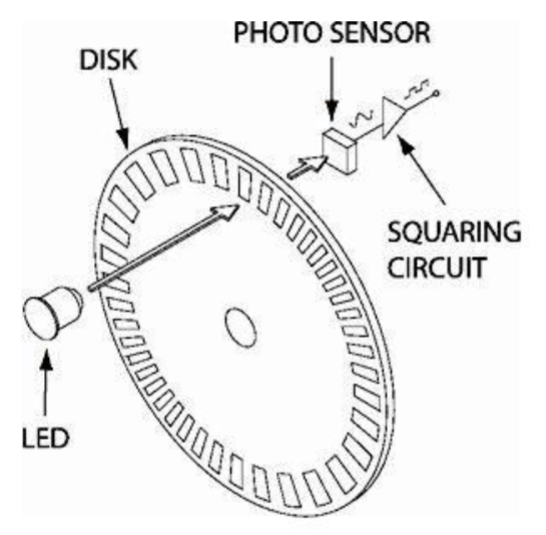
\includegraphics[scale=0.35]{Images/x50_encoder.png}
    \end{center}

    In practice, all optical encoders utilize two offset photosensors, and both the rising and falling edge of \textit{each photosensor} are counted, which quadruples the \textit{resolution} of the optical encoder. This method is called \textit{quadrature encoding}, and it produces a resolution, in counts per revolution, of: \[\text{resolution, with quadrature} = 4\cdot \underbrace{\frac{360^\circ}{n}}_\text{base res.}\] where $n$ is the number of slots.
\end{shaded}

There are many examples of analog sensors, including potentiometers (which act as a variable voltage divider) and inertial sensors, such as those in accelerometers (which use a spring-mass configuration to measure force, and therefore acceleration). In general, a discrete signal is still produced as an output, if only from limitations in resolution. An analog-to-digital converter (ADC) produces a \textit{quantized signal}, which is discrete in value but not necessarily in time. The resolution of such a signal depends on whether distinct endpoints need to be represented in the data; the resolution of such a signal with an $n$-bit ADC is given by: \[\text{resolution} = \begin{cases}
    \displaystyle\frac{\text{range}}{2^n}, & \text{not including an extreme}\\
    \\
    \displaystyle\frac{\text{range}}{2^{n}-1}, & \text{both extremes included}
\end{cases}\]

In general, the \textit{sampling rate} is also finite, and therefore a real signal in most mechatronic systems is discrete in both time and value. The \textit{sampling rate} is a frequency, defined as \[f_s = \frac{1}{T_s}\] where $T_s$ is the sampling time interval. The \textbf{Nyquist condition} gives a minimum sampling frequency to reconstruct a sine wave; since any periodic signal can be decomposed into sine waves, the Nyquist condition applies to any signal which must be sampled, at the \textit{fastest frequency component} $f_{max}$ in the signal. This minimum sampling criteria is given by: \[f_s > f_{s,min} = 2f_{max} \tag{Nyquist Frequency}\] Note that one must sample \textit{faster} than $f_{s,min}$ to meet this condition. If sampling is carried out at exactly $f_{s,min}$, a phase offset can produce a constant signal. In general, sampling too slowly can result in measuring a signal at a \textit{lower} frequency than reality, which is known as \textbf{aliasing}.

Many mechatronic controllers take advantage of numerical differentiation, such as when calculating speed from position data (as may occur with a motor and optical encoder). Note that the speed resolution is given by \[\text{speed resolution} = \frac{\text{position resolution}}{T_s}\] Note that sampling too quickly, i.e. sampling at small intervals $T_s$, actually produces a \textit{poorer} speed resolution. In practice, noise from frequent sampling does indeed contribute to poor results in numerical differentiation; the solution here is either to apply a filter, or to sample less frequently.

A \textit{digital to analog converter}, or DAC, is used to convert discrete digital signals into piecewise-continuous signals (i.e. continuous in time, but quantized in value). An \textit{analog filter} must be used to smooth out the discontinuous jumps. One example of this is \textit{pulse width modulation}, or PWM, which is implemented frequently in motor control. Motors are frequently controlled using a PWM digital to analog conversion. The idea is to alternate rapidly between high- and low- pulses, with a \textit{duty cycle} such that the average voltage is the desired voltage. The duty cycle is the ratio of $t_{on}/t_{total}$.

The motor itself acts as the low-pass filter; since the mechanical components of the motor cannot respond instantaneously, they filter out the rapid changes in supplied voltage and produce a smooth, continuous motion.

PWM signals are amplified with transistors, which operate with $100\%$ theoretical efficiency. In practice, PWM signals have very high efficiencies, in excess of $90\%$. This is the benefit of PWM signals over other methods for producing a voltage drop, such as increasing resistance.

\begin{shaded}
    \textbf{Types of Control}. There are two general schemes for control, both of which are frequently utilized and come with their own advantages and disadvantages:
    \begin{enumerate}
        \item[] \textbf{Feedforward (Open-Loop) Control}. Feedforward control refers to a control law which does not depend on any external signals. In general, feedforward control is preset on a controller based on observations or models, and it cannot adjust if these assumptions change during operation. Common examples include offsets (i.e. a fixed voltage output to overcome friction, a fixed setpoint to overcome gravity, etc). Feedforward control is the most common type of control because it is inexpensive, simple, and does not require sensors.
        \item[] \textbf{Feedback (Closed-Loop) Control}. Feedback control refers to a control law which adjusts its output depending on external signals. Feedback control is able to respond to changes detected by the system's sensors, often utilizing microcontrollers for this purpose. The disadvantage of these control laws is that they are reactive, requiring an external signal before they can act. A common example is PID control, or any of its variants (P, PI, etc).
    \end{enumerate}
    Feedforward and feedback control can be, and frequently are, combined. For example, motor control may be performed using PID control with a constant friction compensation voltage. Such a scheme allows the feedback loop to react faster, because less windup is necessary to reach the required voltage to prescribe motion.
\end{shaded}

\subsection{Constraint of Motion}

This section is dedicated to an analysis of mechanical devices which constrain motion. In particular, the failure conditions for fasteners and bearings will be discussed.

For a bolt of stiffness $k_b$ and a clamped member of stiffness $k_m$, define the joint constant to be: \[C:= \frac{k_b}{k_b+k_m}\] If $P$ is the external load on the joint, and $F_i$ is the preload from tightening the bolt, the force $F_b$ in the joining bolt can be calculated, as long as the joint does not separate, as follows: \[F_b = \underbrace{\frac{k_b}{k_b+k_m}}_C P +F_i\] Standard recommendations for preload are a function of the fastener's area, $A_t$, and the fastener's proof strength, $S_p$. Common guidance is \[F_i = \begin{cases}
    0.75S_p A_t, & \text{temporary connections}\\
    0.9S_pA_t, & \text{permanent connections}
\end{cases}\] It is much more practical to specify a target pre-load torque, $T$, which can be attained with a torque wrench or similar device. The recommended target torque is a function of the desired preload, the major diameter $d$ of the fastener, and an empirical proportionality constant, which is typically $K\approx 0.2$ for most applications. Then, the torque which produces the desired preload $F_i$ is given by: \[T = KF_i d\] There are several failure modes for a joint, each of which has an associated factor of safety. First is the factor of safety against joint seperation, $n_s$, which is given by \[n_s = \frac{F_i}{(1-C)P}\tag{Safety Factor of Separation}\] Fatigue failure can be predicted with Goodman's rule, and the factor of safety against fatigue failure, $n_f$, is a function of the load, as well as ultimate tensile strength $S_{ut}$ and the endurance strength $S_e$, which are material properties: \[n_f = \frac{2}{C}\cdot \frac{S_{ut}A_t-F_i}{P+\frac{S_{ut}}{S_e}P}\tag{Safety Factor of Fatigue}\] Finally, the safety factor $n_L$ for yield is given by: \[n_L = \frac{1}{C}\cdot \frac{S_pA_t-F_i}{P}\tag{Safety Factor of Yield}\]

Besides fasteners, \textit{bearings}, including ball bearings and roller bearings, are common elements in many mechanical designs. The calculation of bearing life under given load conditions involves empirical data, typically from a manufacturer catalog. The load rating for \textbf{90\% reliability under a given, \textit{purely radial} load $F_D$}, is given by the relationship: \[C_{10} = F_D \left(\frac{L_D}{L_R}\right)^a\tag{$90\%$ reliability}\] where $a=\begin{cases}
    1/3, & \text{ball bearings}\\
    3/10, & \text{roller bearings}
\end{cases}$, $L_D$ is the desired lifetime in revolutions, and $L_R$ is the rated lifetime, which is typically $10^6$ revolutions. If $F_D$, $L_D$, and $a$ are known, taking $L_R=10^6$ allows one to select any bearing from a catalog with a $C_{10}$ greater than the calculated $C_{10}$ value to ensure $90\%$ reliability under the given radial loading conditions. If a greater reliability is desired, one can use the general formula for the $C_{10}$ rating, which is a Weibull distribution: \[C_{10} := a_f F_D \left[\frac{L_D/L_R}{x_0+(\theta-x_0)(1-R_D)^{1/b}}\right]^a\] where $a$ is as before, and $R_D\geq 0.9$ is the desired reliability. The parameters $x_0$, $\theta$, and $b$ are Weibull parameters which a manufacturer may report, and $a_f$ is a factor of safety.

\begin{shaded}
\textbf{Calculation of Equivalent Loads}. Note that these relationships are only valid for radial load $F_D$. If there is an axial component to the force, one must first compute the equivalent load $F_e$ which would be felt if the load were purely radial. The general steps for computing this equivalent load are as follows: \begin{enumerate}
    \item[1.] Use a catalog to find a value for $C_0$, which corresponds uniquely either to the bearing size.
    \item[2.] Calculate $F_a/C_0$, the ratio of axial load to $C_0$. Use this value with a catalog to estimate the \textit{limiting load ratio} $e$, which should be tabulated and correspond uniquely to $F_a/C_0$.
    \item[3.] Let $V=\begin{cases}
        1,\ & \text{inner ring rotation}\\
        1.2, & \text{outer ring rotation}
    \end{cases}$. If $e\leq F_a/(VF_r)$, where $F_r$ is the axial load, then $F_e\approx VF_r$. If $F_a/(VF_r)> e$, then $F_e$ is calculated by the following empirical relationship: \[F_e = 0.56 V F_r + Y F_a\] where $Y$ is the empirical relating slope, and its value is read from the catalog.
\end{enumerate}
\end{shaded}

Note that this process requires that the bearing size is specified, as this is how $C_0$ was determined. One can work backwards, from a guess satisfying $F_a/(VF_r)>e$, to determine $C_{10}$, and this process can be performed iteratively until a suitable bearing is selected.